% options:
% thesis=B bachelor's thesis
% thesis=M master's thesis
% czech thesis in Czech language
% slovak thesis in Slovak language
% english thesis in English language
% hidelinks remove colour boxes around hyperlinks

\documentclass[thesis=M,english]{FITthesis}[2012/06/26]

\usepackage[utf8]{inputenc} % LaTeX source encoded as UTF-8

\usepackage{graphicx} %graphics files inclusion
% \usepackage{amsmath} %advanced maths
% \usepackage{amssymb} %additional math symbols

\usepackage{dirtree} %directory tree visualisation

% % list of acronyms


\usepackage[acronym,nonumberlist,toc,numberedsection=autolabel]{glossaries}
\iflanguage{english}{\renewcommand*{\acronymname}{List of abbreviations used}}{}
\makeglossaries

\usepackage{todonotes}
\usepackage{enumitem}
\usepackage{hyperref}
\usepackage{tabularx}
\usepackage{spverbatim}
\usepackage{listings}
\usepackage{caption}

\DeclareCaptionFont{white}{\color{white}}
\DeclareCaptionFormat{listing}{\colorbox{gray}{\parbox{\textwidth}{#1#2#3}}}
\captionsetup[lstlisting]{format=listing,labelfont=white,textfont=white}

\newcommand{\tg}{\mathop{\mathrm{tg}}} %cesky tangens
\newcommand{\cotg}{\mathop{\mathrm{cotg}}} %cesky cotangens

\department{Katedra \ldots softwarového inženýrství}
\title{A Case Study and Proof of Concept of the Application of Machine Learning to Polarion's ALM Software}
\authorGN{Michal} %(křestní) jméno (jména) autora
\authorFN{Sláma} %příjmení autora
\authorWithDegrees{Bc. Michal Sláma} %jméno autora včetně současných akademických titulů
\author{Jan Nový} %jméno autora bez akademických titulů
\supervisor{Ing. Jurij Černikov}
\acknowledgements{I would like to thank to my supervisour for his extraordinary leading and valuable advices during the whole process of writing this thesis.}
\abstractCS{Machine learning (ML) is becaming essencial part any software application. Its same for application lifecycle management (ALM) which hides great opportunities to improve using, processing or behaviour of the whole system based on the ML principies. This work cointains description of ML principies relevat for using in the ALM environment. For the specific software is used Polarion which is wordwide successful enterprise solution for ALM. This thesis provides analysis it's core business and user cases and posible ways how to integrate ML to improve Polarion in different areas. As Polarion must that customer's data are not exposed to any possible thread ensure on all levels we will discuss the way how to achieve this goal by a different kind of architecture or implementation. }
\abstractEN{Sem doplňte ekvivalent abstraktu Vaší práce v~angličtině.}
\placeForDeclarationOfAuthenticity{V~Praze}
\declarationOfAuthenticityOption{4} %volba Prohlášení (číslo 1-6)
\keywordsCS{Strojové učení, životní cyklus softwarových aplikací, ALM}
\keywordsEN{Machine learning, application lifecycle management, ALM}

%definition for Java source code examples
\lstset{
	basicstyle=\footnotesize\ttfamily,
	numberstyle=\tiny,
	numbersep=5pt,
	tabsize=2,
	extendedchars=true,
	breaklines=true,
	%	showstringspaces=true,
	keywordstyle=\color{red},
	frame=b,         
	stringstyle=\color{white}\ttfamily,
	showspaces=false, 
	showtabs=false,  
	xleftmargin=17pt,
	framexleftmargin=17pt,
	framexrightmargin=5pt,
	framexbottommargin=4pt,
	showstringspaces=false, 
	breakatwhitespace=true,
	commentstyle=\color{pgreen},
	keywordstyle=\color{pblue},
	stringstyle=\color{pred}    
}
\lstloadlanguages{Java}

\begin{document}


\newacronym{alm}{ALM}{Application lifecycle management}
\newacronym{ml}{ML}{Machine learning}
\newacronym{polarion}{Polarion}{Polarion ALM} 

\todototoc
\listoftodos

\begin{introduction}
\begin{center}
	\textit{\textit{The revolution is just beginning, but it’s real – and the time to act is now. In fact, it is yours for the taking to harness a broad platform, services and ecosystem to transform your business. A unified approach to application lifecycle management is not a futuristic technology trend. It’s here today,and the good news is that you don’t have to completely stop and reset, but can smoothly transition from squeezing the most out of your existing business processes to making your organization thrive.}}\\
Kurt Bittner\\
Analyst\\
Forrester Research\\
\end{center}
\end{introduction}


We live in the world that is changing rapidly. No part of life of free to this changes and the software development needs more then others to adapt every day to new requirements and technologies. This demand leads to a new level of management for software development where tools, process, implementation, testing and reporting are organized on one place with goal to keep and improve traceability and productivity as high as possible. This comes hand by hand with automation in the form of \acrshort{ml} that moves user experience and reporting to the next level. One of such product is \acrshort{polarion}\cite{polarion_alm} and this work will analyze it's user cases and find out what places are good candidates for using \acrshort{ml} techniques to improve business value of the product. 

\chapter{The aim of the thesis}

sThe aim of this thesis is to analyze and identify machine learning (\acrshort{ml}) use cases that would prove valuable for \acrshort{polarion}’s application lifecycle management (\acrshort{alm}) software. A proof of concept prototype will be supplied for the selected use case.

\begin{enumerate}[nosep]
	\item Analyze and describe \acrshort{polarion} in order to identify suitable use cases to apply ML to. 
	\item Provide a review of ML frameworks and algorithms that are relevant for such an application.
	\item Describe several use cases for ML and define their benefit to both \acrshort{alm} as a business and the users that deploy it.
	\item Choose a scenario from the previous investigation and implement a proof of concept prototype.
	\item Discuss the possibility of the full implementation and deployment of the previous prototype into the production environment.
\end{enumerate}

\chapter{Polarion}

Organizations must accelerate innovation to stay competitive
in most industries. Unlocking team synergies across disparate
software development teams is paramount. Many organizations
are still struggling with the old way of doing things.
They focus on isolated process optimization instead of driving
business value through comprehensive synchronization. With
Polarion ALM, customers have been able to get their teams
out of their silos and orchestrate development efforts across
the entire application lifecycle. This approach has empowered
stakeholders to better perform tasks in context and quickly
make sound decisions based on real-time access to
information.


Siemens PLM Software, a business unit of the Siemens
Digital Factory Division, is a leading global provider of
product lifecycle management (PLM) and manufacturing
operations management (MOM) software, systems and
services with over 15 million licensed seats and more than
140,000 customers worldwide. Headquartered in Plano,
Texas, Siemens PLM Software works collaboratively with its
customers to provide industry software solutions that help
companies everywhere achieve a sustainable competitive
advantage by making real the innovations that matter. For
more information on Siemens PLM Software products and
services, visit www.siemens.com/plm.

\section{ALM}

\section{Reporting}

\section{Using}

\subsection{Licenses}

\chapter{Machine learning}

\section{Frameworks}

\subsection{TensorFlow}

\subsection{Theano}

\subsection{Caffe}

\subsection{AML - AWS}

\subsection{Microsoft CNTK}

\section{Algorithms}

\subsection{LDA}

\chapter{Creating work items with ML}

\section{User experience}

\section{Architecture}

\section{Realization of prototype}

\chapter{ML in production environment}

\chapter{Security}

implement own ML server using just shareable libraries and provides to customers ability to using ML technics.

\chapter{Validity}

\chapter{The value of the enhancement}

\begin{conclusion}
	%sem napište závěr Vaší práce
\end{conclusion}

\bibliographystyle{csn690}
\bibliography{mybibliographyfile}

\appendix

\chapter{List of abbreviations used}

\printglossaries

\begin{description}
	\item[ALM] Application lifecycle management
	\item[Polarion] Polarion ALM
	\item[ML] Machine learning 
\end{description}


% % % % % % % % % % % % % % % % % % % % % % % % % % % % 
% % Tuto kapitolu z výsledné práce ODSTRAŇTE.
% % % % % % % % % % % % % % % % % % % % % % % % % % % % 
% 
% \chapter{Návod k~použití této šablony}
% 
% Tento dokument slouží jako základ pro napsání závěrečné práce na Fakultě informačních technologií ČVUT v~Praze.
% 
% \section{Výběr základu}
% 
% Vyberte si šablonu podle druhu práce (bakalářská, diplomová), jazyka (čeština, angličtina) a kódování (ASCII, \mbox{UTF-8}, \mbox{ISO-8859-2} neboli latin2 a nebo \mbox{Windows-1250}). 
% 
% V~české variantě naleznete šablony v~souborech pojmenovaných ve formátu práce\_kódování.tex. Typ může být:
% \begin{description}
% 	\item[BP] bakalářská práce,
% 	\item[DP] diplomová (magisterská) práce.
% \end{description}
% Kódování, ve kterém chcete psát, může být:
% \begin{description}
% 	\item[UTF-8] kódování Unicode,
% 	\item[ISO-8859-2] latin2,
% 	\item[Windows-1250] znaková sada 1250 Windows.
% \end{description}
% V~případě nejistoty ohledně kódování doporučujeme následující postup:
% \begin{enumerate}
% 	\item Otevřete šablony pro kódování UTF-8 v~editoru prostého textu, který chcete pro psaní práce použít -- pokud můžete texty s~diakritikou normálně přečíst, použijte tuto šablonu.
% 	\item V~opačném případě postupujte dále podle toho, jaký operační systém používáte:
% 	\begin{itemize}
% 		\item v~případě Windows použijte šablonu pro kódování \mbox{Windows-1250},
% 		\item jinak zkuste použít šablonu pro kódování \mbox{ISO-8859-2}.
% 	\end{itemize}
% \end{enumerate}
% 
% 
% V~anglické variantě jsou šablony pojmenované podle typu práce, možnosti jsou:
% \begin{description}
% 	\item[bachelors] bakalářská práce,
% 	\item[masters] diplomová (magisterská) práce.
% \end{description}
% 
% \section{Použití šablony}
% 
% Šablona je určena pro zpracování systémem \LaTeXe{}. Text je možné psát v~textovém editoru jako prostý text, lze však také využít specializovaný editor pro \LaTeX{}, např. Kile.
% 
% Pro získání tisknutelného výstupu z~takto vytvořeného souboru použijte příkaz \verb|pdflatex|, kterému předáte cestu k~souboru jako parametr. Vhodný editor pro \LaTeX{} toto udělá za Vás. \verb|pdfcslatex| ani \verb|cslatex| \emph{nebudou} s~těmito šablonami fungovat.
% 
% Více informací o~použití systému \LaTeX{} najdete např. v~\cite{wikilatex}.
% 
% \subsection{Typografie}
% 
% Při psaní dodržujte typografické konvence zvoleného jazyka. České \uv{uvozovky} zapisujte použitím příkazu \verb|\uv|, kterému v~parametru předáte text, jenž má být v~uvozovkách. Anglické otevírací uvozovky se v~\LaTeX{}u zadávají jako dva zpětné apostrofy, uzavírací uvozovky jako dva apostrofy. Často chybně uváděný symbol "{} (palce) nemá s~uvozovkami nic společného.
% 
% Dále je třeba zabránit zalomení řádky mezi některými slovy, v~češtině např. za jednopísmennými předložkami a spojkami (vyjma \uv{a}). To docílíte vložením pružné nezalomitelné mezery -- znakem \texttt{\textasciitilde}. V~tomto případě to není třeba dělat ručně, lze použít program \verb|vlna|.
% 
% Více o~typografii viz \cite{kobltypo}.
% 
% \subsection{Obrázky}
% 
% Pro umožnění vkládání obrázků je vhodné použít balíček \verb|graphicx|, samotné vložení se provede příkazem \verb|\includegraphics|. Takto je možné vkládat obrázky ve formátu PDF, PNG a JPEG jestliže používáte pdf\LaTeX{} nebo ve formátu EPS jestliže používáte \LaTeX{}. Doporučujeme preferovat vektorové obrázky před rastrovými (vyjma fotografií).
% 
% \subsubsection{Získání vhodného formátu}
% 
% Pro získání vektorových formátů PDF nebo EPS z~jiných lze použít některý z~vektorových grafických editorů. Pro převod rastrového obrázku na vektorový lze použít rasterizaci, kterou mnohé editory zvládají (např. Inkscape). Pro konverze lze použít též nástroje pro dávkové zpracování běžně dodávané s~\LaTeX{}em, např. \verb|epstopdf|.
% 
% \subsubsection{Plovoucí prostředí}
% 
% Příkazem \verb|\includegraphics| lze obrázky vkládat přímo, doporučujeme však použít plovoucí prostředí, konkrétně \verb|figure|. Například obrázek \ref{fig:float} byl vložen tímto způsobem. Vůbec přitom nevadí, když je obrázek umístěn jinde, než bylo původně zamýšleno -- je tomu tak hlavně kvůli dodržení typografických konvencí. Namísto vynucování konkrétní pozice obrázku doporučujeme používat odkazování z~textu (dvojice příkazů \verb|\label| a \verb|\ref|).
% 
% \begin{figure}\centering
% 	
\includegraphics[width=0.5\textwidth, angle=30]{cvut-logo-bw}
% 	\caption[Příklad obrázku]{Ukázkový obrázek v~plovoucím prostředí}\label{fig:float}
% \end{figure}
% 
% \subsubsection{Verze obrázků}
% 
% % Gnuplot BW i barevně
% Může se hodit mít více verzí stejného obrázku, např. pro barevný či černobílý tisk a nebo pro prezentaci. S~pomocí některých nástrojů na generování grafiky je to snadné.
% 
% Máte-li například graf vytvořený v programu Gnuplot, můžete jeho černobílou variantu (viz obr. \ref{fig:gnuplot-bw}) vytvořit parametrem \verb|monochrome dashed| příkazu \verb|set term|. Barevnou variantu (viz obr. \ref{fig:gnuplot-col}) vhodnou na prezentace lze vytvořit parametrem \verb|colour solid|.
% 
% \begin{figure}\centering
% 	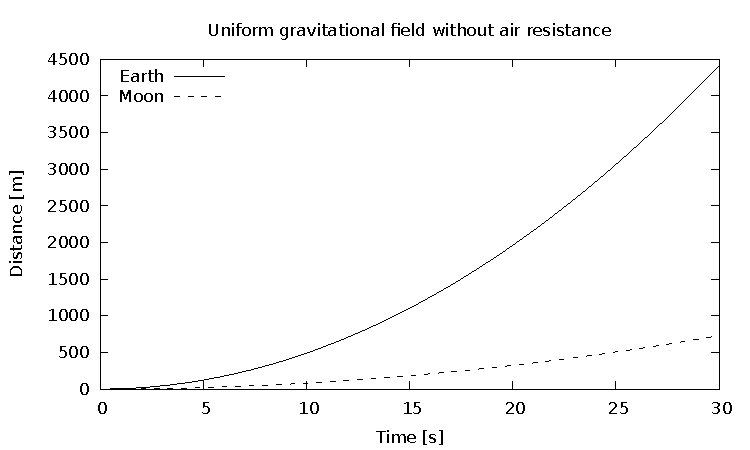
\includegraphics{gnuplot-bw}
% 	\caption{Černobílá varianta obrázku generovaného programem Gnuplot}\label{fig:gnuplot-bw}
% \end{figure}
% 
% \begin{figure}\centering
% 	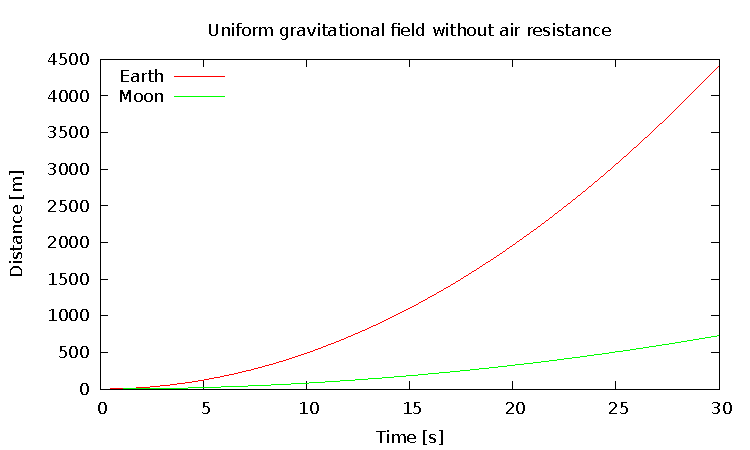
\includegraphics{gnuplot-col}
% 	\caption{Barevná varianta obrázku generovaného programem Gnuplot}\label{fig:gnuplot-col}
% \end{figure}
% 
% 
% \subsection{Tabulky}
% 
% Tabulky lze zadávat různě, např. v~prostředí \verb|tabular|, avšak pro jejich vkládání platí to samé, co pro obrázky -- použijte plovoucí prostředí, v~tomto případě \verb|table|. Například tabulka \ref{tab:matematika} byla vložena tímto způsobem.
% 
% \begin{table}\centering
% 	\caption[Příklad tabulky]{Zadávání matematiky}\label{tab:matematika}
% 	\begin{tabular}{|l|l|c|c|}\hline
% 		Typ		& Prostředí		& \LaTeX{}ovská zkratka	& \TeX{}ovská zkratka	\tabularnewline \hline \hline
% 		Text		& \verb|math|		& \verb|\(...\)|	& \verb|$...$|		\tabularnewline \hline
% 		Displayed	& \verb|displaymath|	& \verb|\[...\]|	& \verb|$$...$$|	\tabularnewline \hline
% 	\end{tabular}
% \end{table}
% 
% % % % % % % % % % % % % % % % % % % % % % % % % % % % 

\chapter{CD contains}

\begin{figure}
	\dirtree{%
		.1 readme.txt\DTcomment{stručný popis obsahu CD}.
		.2 thesis\DTcomment{zdrojová forma práce ve formátu \LaTeX{}}.
		.1 text\DTcomment{text práce}.
		.2 thesis.pdf\DTcomment{text práce ve formátu PDF}.
		.2 thesis.ps\DTcomment{text práce ve formátu PS}.
	}
\end{figure}

\end{document}
